\section{Control Unit}
The datapath derived from figure \autoref{fig:iir-dfd} requires two control signals to clear all registers and to enable the latch. A single status signal \texttt{VOUT} must be provided, as requested. The resulting ASM chart describing the state machine is in figure \autoref{fig:asm}.
\todo{Consider if anything is missing regarding CU}
\todo{Can the image be smaller? It might fit under this text given how short it is}
\begin{figure}
		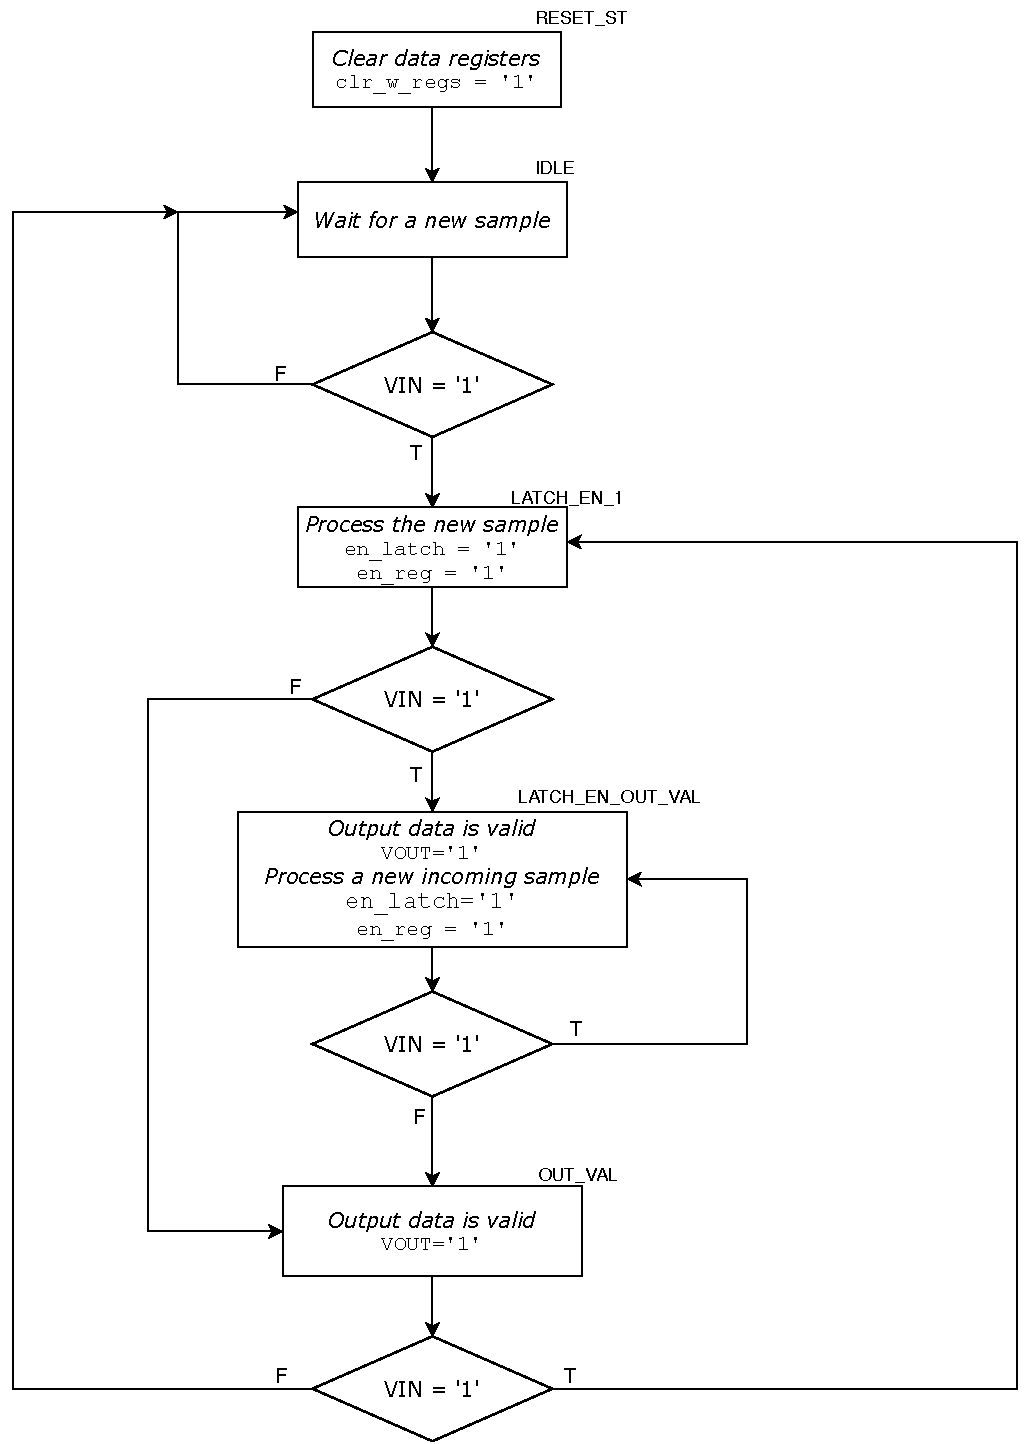
\includegraphics[width=\textwidth]{./chapter2/images/asm_standard.pdf}
		\caption{ASM chart representing the state machine for the standard architecture. The values of the control signals are indicated along with comments describing the purpose of each state}
		\label{fig:asm}
\end{figure}
